\subsubsection{LCA - Lowest Common Ancestor (Menor Ancestral Comum)}
O LCA de dois nós $u$ e $v$ em uma árvore enraizada é o nó mais profundo que é
ancestral de ambos. O método de \textit{Binary Lifting} (Içamento Binário)
pré-calcula os ancestrais de potências de 2 em $\mathcal{O}(N \log N)$,
permitindo responder a cada consulta de LCA em $\mathcal{O}(\log N)$.

Veja o LCA por Içamento Binário em ação:\\ \vspace{0.5cm} \noindent
\begin{minipage}[t]{0.31\textwidth}
    \centering
    \textbf{Passo 1: Árvore Enraizada}\\
    \vspace{0.2cm}
    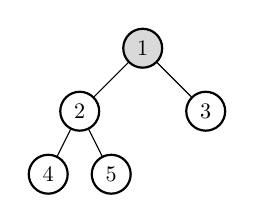
\begin{tikzpicture}[every node/.style={circle, draw, minimum size=0.5cm, thick}, scale=0.8, every node/.append style={transform shape}, >=stealth]
        \node[fill=gray!30] (1) at (1, 2) {1};
        \node (2) at (0, 1) {2};
        \node (3) at (2, 1) {3};
        \node (4) at (-0.5, 0) {4};
        \node (5) at (0.5, 0) {5};
        \draw (1) -- (2);
        \draw (1) -- (3);
        \draw (2) -- (4);
        \draw (2) -- (5);
    \end{tikzpicture}

    \vspace{0.2cm}
    \footnotesize
    \raggedright
    Árvore com 5 nós. O nó 1 é definido como a raiz.
\end{minipage}%
\hfill
%
\begin{minipage}[t]{0.31\textwidth}
    \centering
    \textbf{Passo 2: Pré-cálculo ($up$)}\\
    \vspace{0.2cm}
    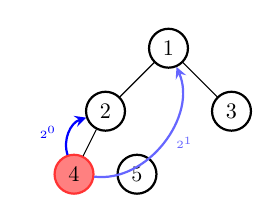
\begin{tikzpicture}[every node/.style={circle, draw, minimum size=0.5cm, thick}, scale=0.8, every node/.append style={transform shape}, >=stealth]
        \node (1) at (1, 2) {1};
        \node (2) at (0, 1) {2};
        \node (3) at (2, 1) {3};
        \node[fill=red!50, draw=red!80] (4) at (-0.5, 0) {4};
        \node (5) at (0.5, 0) {5};
        \draw (1) -- (2);
        \draw (1) -- (3);
        \draw (2) -- (4);
        \draw[->, blue, thick, bend left=45] (4) to node[left, draw=none, fill=none] {\tiny $2^0$} (2);
        \draw[->, blue!60, thick, bend right=60] (4) to node[right, draw=none, fill=none] {\tiny $2^1$} (1);
    \end{tikzpicture}

    \vspace{0.2cm}
    \footnotesize
    \raggedright
    Armazena ancestrais de potências de 2 ($up[4][0]=2, up[4][1]=1$).
\end{minipage}%
\hfill
%
\begin{minipage}[t]{0.31\textwidth}
    \centering
    \textbf{Passo 3: Consulta de LCA}\\
    \vspace{0.2cm}
    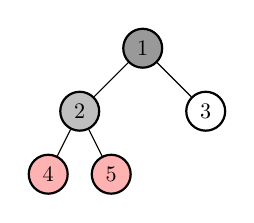
\begin{tikzpicture}[every node/.style={circle, draw, minimum size=0.5cm, thick}, scale=0.8, every node/.append style={transform shape}, >=stealth]
        \node[fill=gray!80] (1) at (1, 2) {1};
        \node[fill=gray!50] (2) at (0, 1) {2};
        \node (3) at (2, 1) {3};
        \node[fill=red!30] (4) at (-0.5, 0) {4};
        \node[fill=red!30] (5) at (0.5, 0) {5};
        \draw (1) -- (2);
        \draw (1) -- (3);
        \draw (2) -- (4);
        \draw (2) -- (5);
    \end{tikzpicture}

    \vspace{0.2cm}
    \footnotesize
    \raggedright
    O LCA entre os nós 4 e 5 é o nó 2 (ancestral comum mais profundo).
\end{minipage}

\vspace{0.3cm}

\paragraph{Implementação: }\mbox{}\\
\textbf{C++:}
\begin{lstlisting}[language=C++]
int n, l;
vector<vector<int>> adj;
vector<vector<int>> up;
vector<int> tin, tout;
int timer;

void dfs(int v, int p) {
    tin[v] = ++timer;
    up[v][0] = p;
    for (int i = 1; i <= l; ++i)
        up[v][i] = up[up[v][i - 1]][i - 1];
    for (int u : adj[v]) {
        if (u != p) dfs(u, v);
    }
    tout[v] = ++timer;
}

bool is_ancestor(int u, int v) {
    return tin[u] <= tin[v] && tout[u] >= tout[v];
}

int lca(int u, int v) {
    if (is_ancestor(u, v)) return u;
    if (is_ancestor(v, u)) return v;
    for (int i = l; i >= 0; --i) {
        if (!is_ancestor(up[u][i], v))
            u = up[u][i];
    }
    return up[u][0];
}

void preprocess(int root) {
    tin.resize(n); tout.resize(n);
    timer = 0;
    l = ceil(log2(n));
    up.assign(n, vector<int>(l + 1));
    dfs(root, root);
}
\end{lstlisting}
\newpage